\documentclass[../Main.tex]{subfiles}
\begin{document}

\section{Ideas for New Alternative Games}
    \subsection{Background}
    \subsection{Concepts}
        \subsubsection{Hover}
        \blindtext
            
            \begin{figure}[H]
              \centering
              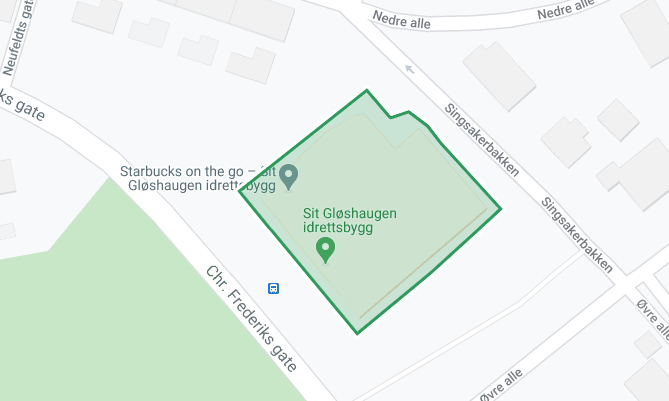
\includegraphics[width=.75\textwidth]{Images/OurConcepts/GeofenceSIT.png}
              \caption{A geofence surrounding Sit Gløshaugen training center in Trondheim.}
              \label{fig:geofence}
            \end{figure}
        \blindtext    
            
            \begin{figure}[H]
              \centering
              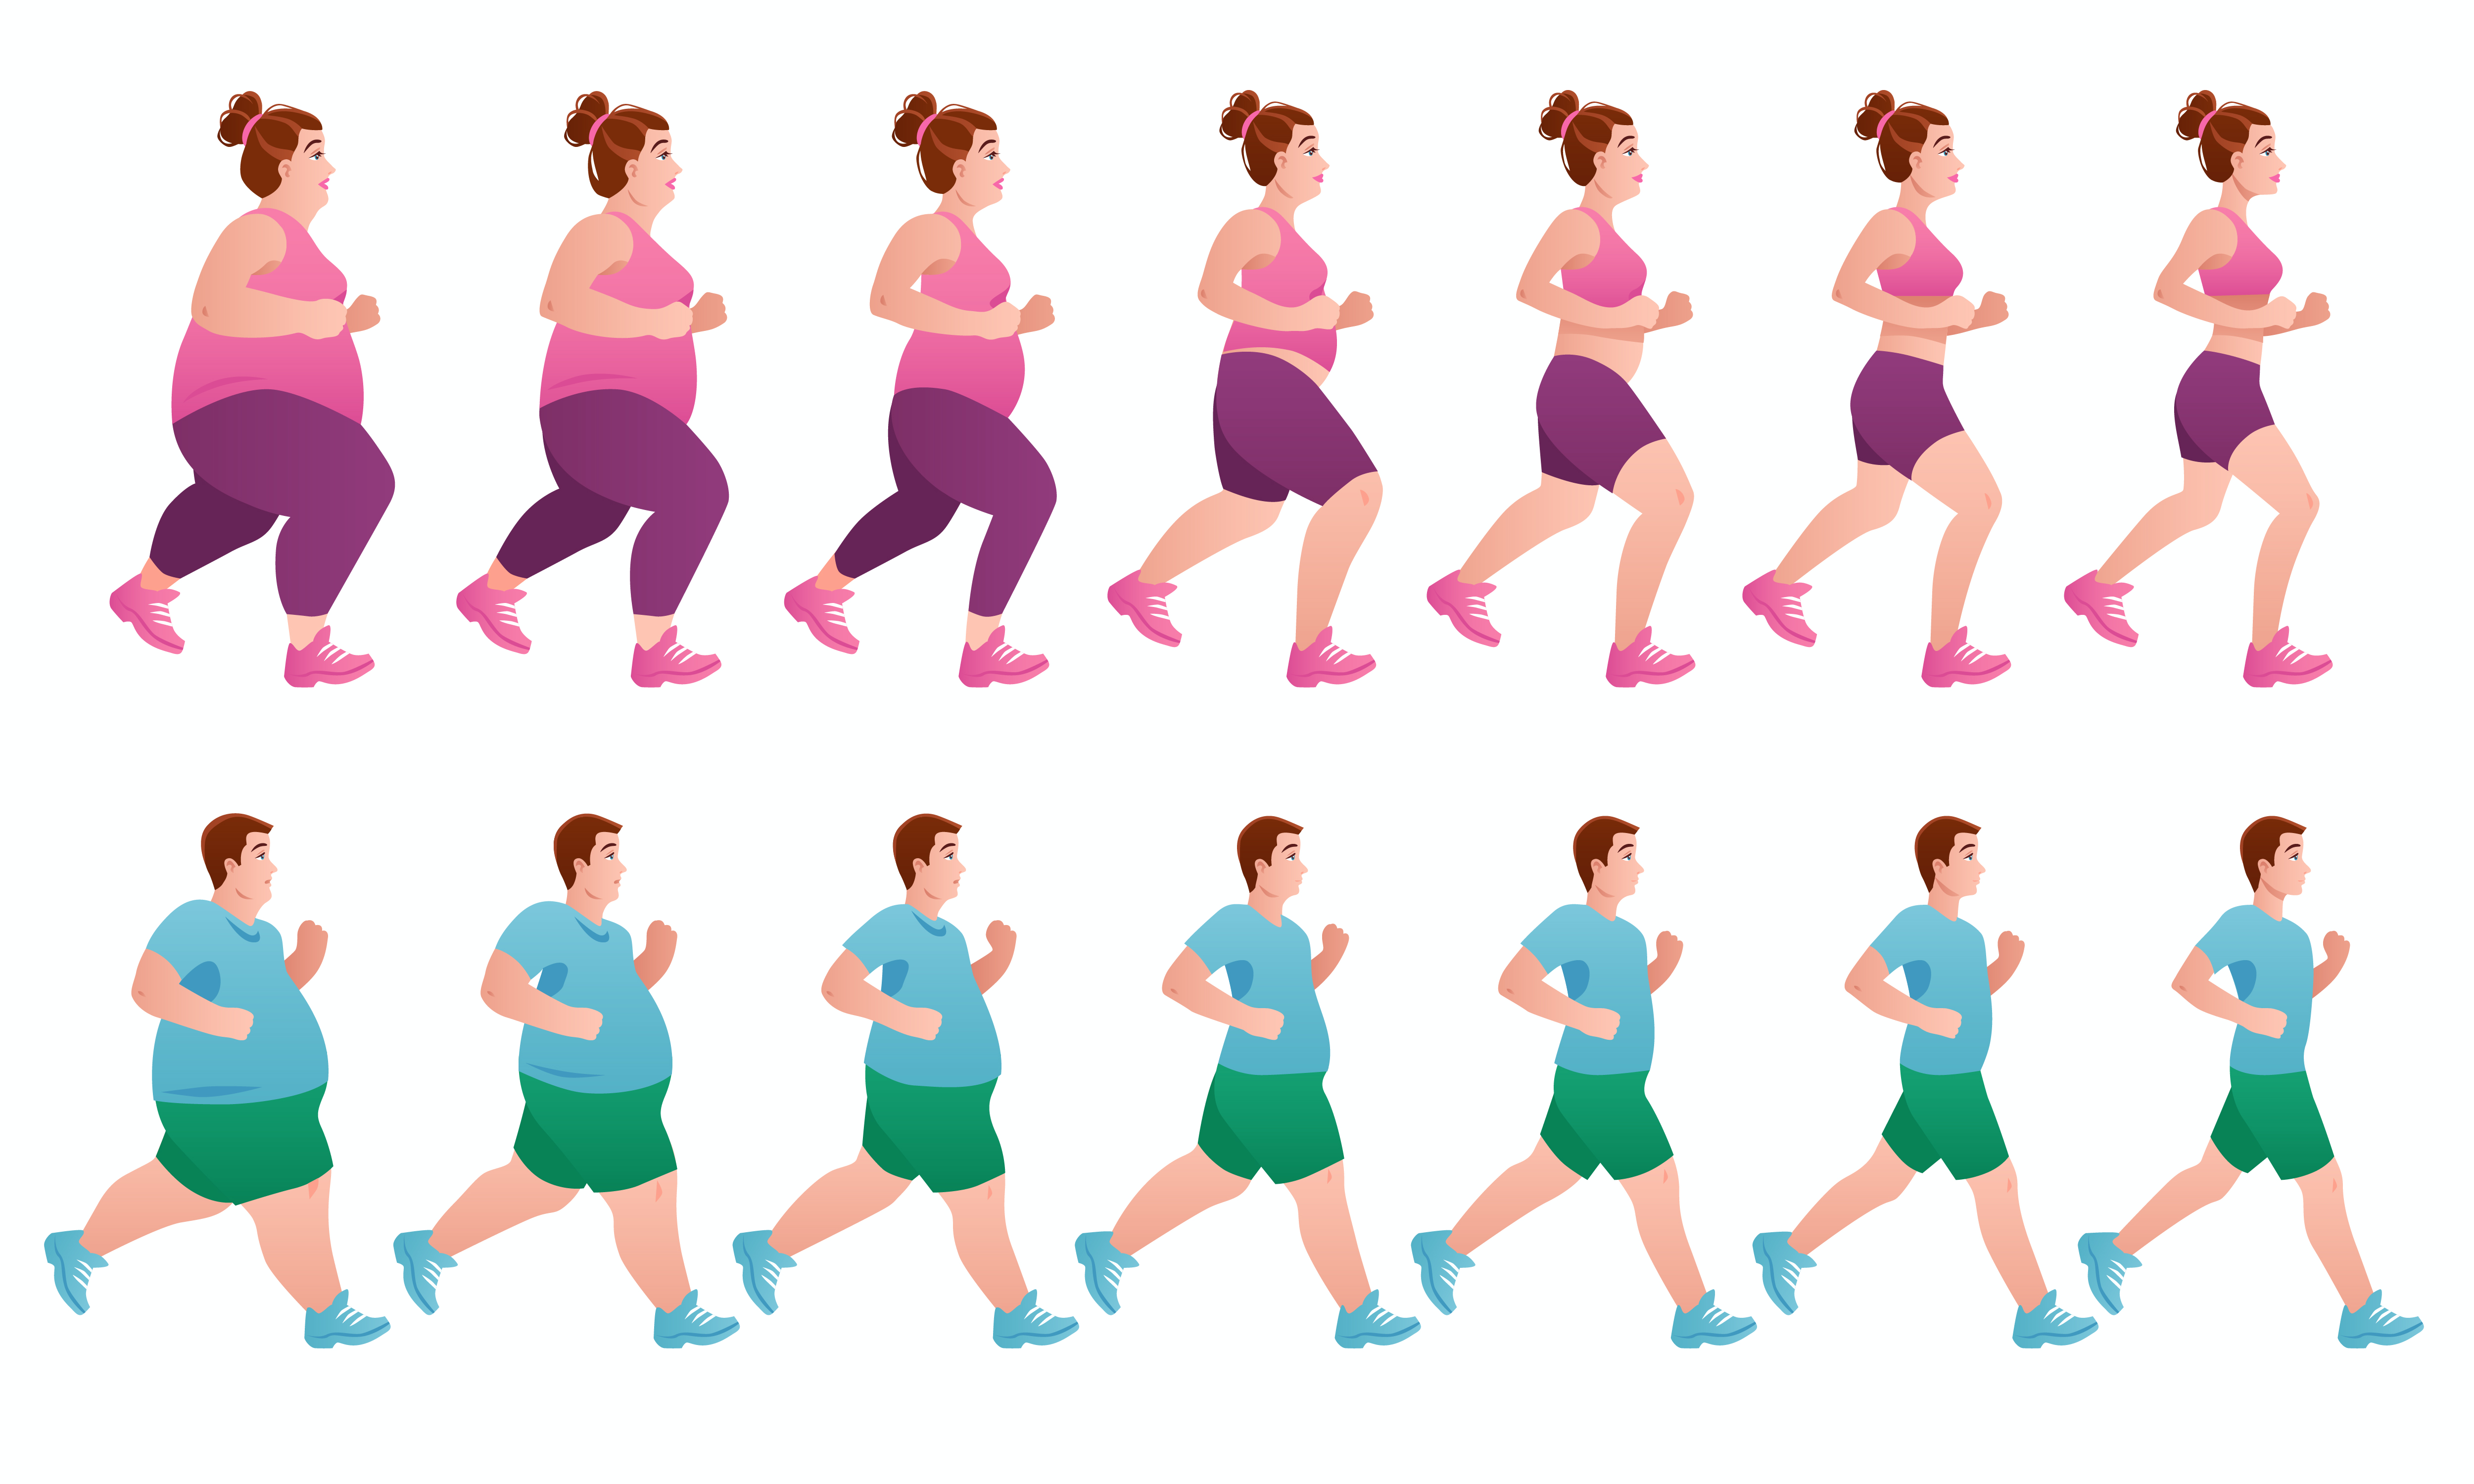
\includegraphics[width=.6\textwidth]{Images/OurConcepts/ExerciseTransformation.png}
              \caption{Example of how the virtual character in Hover could evolve \citep{macrovector_fitness_2020}}
              \label{fig:player_evolement}
            \end{figure}
            
        
        \subsubsection{Guess Where}
            \begin{wrapfigure}{r}{0.5\textwidth}
              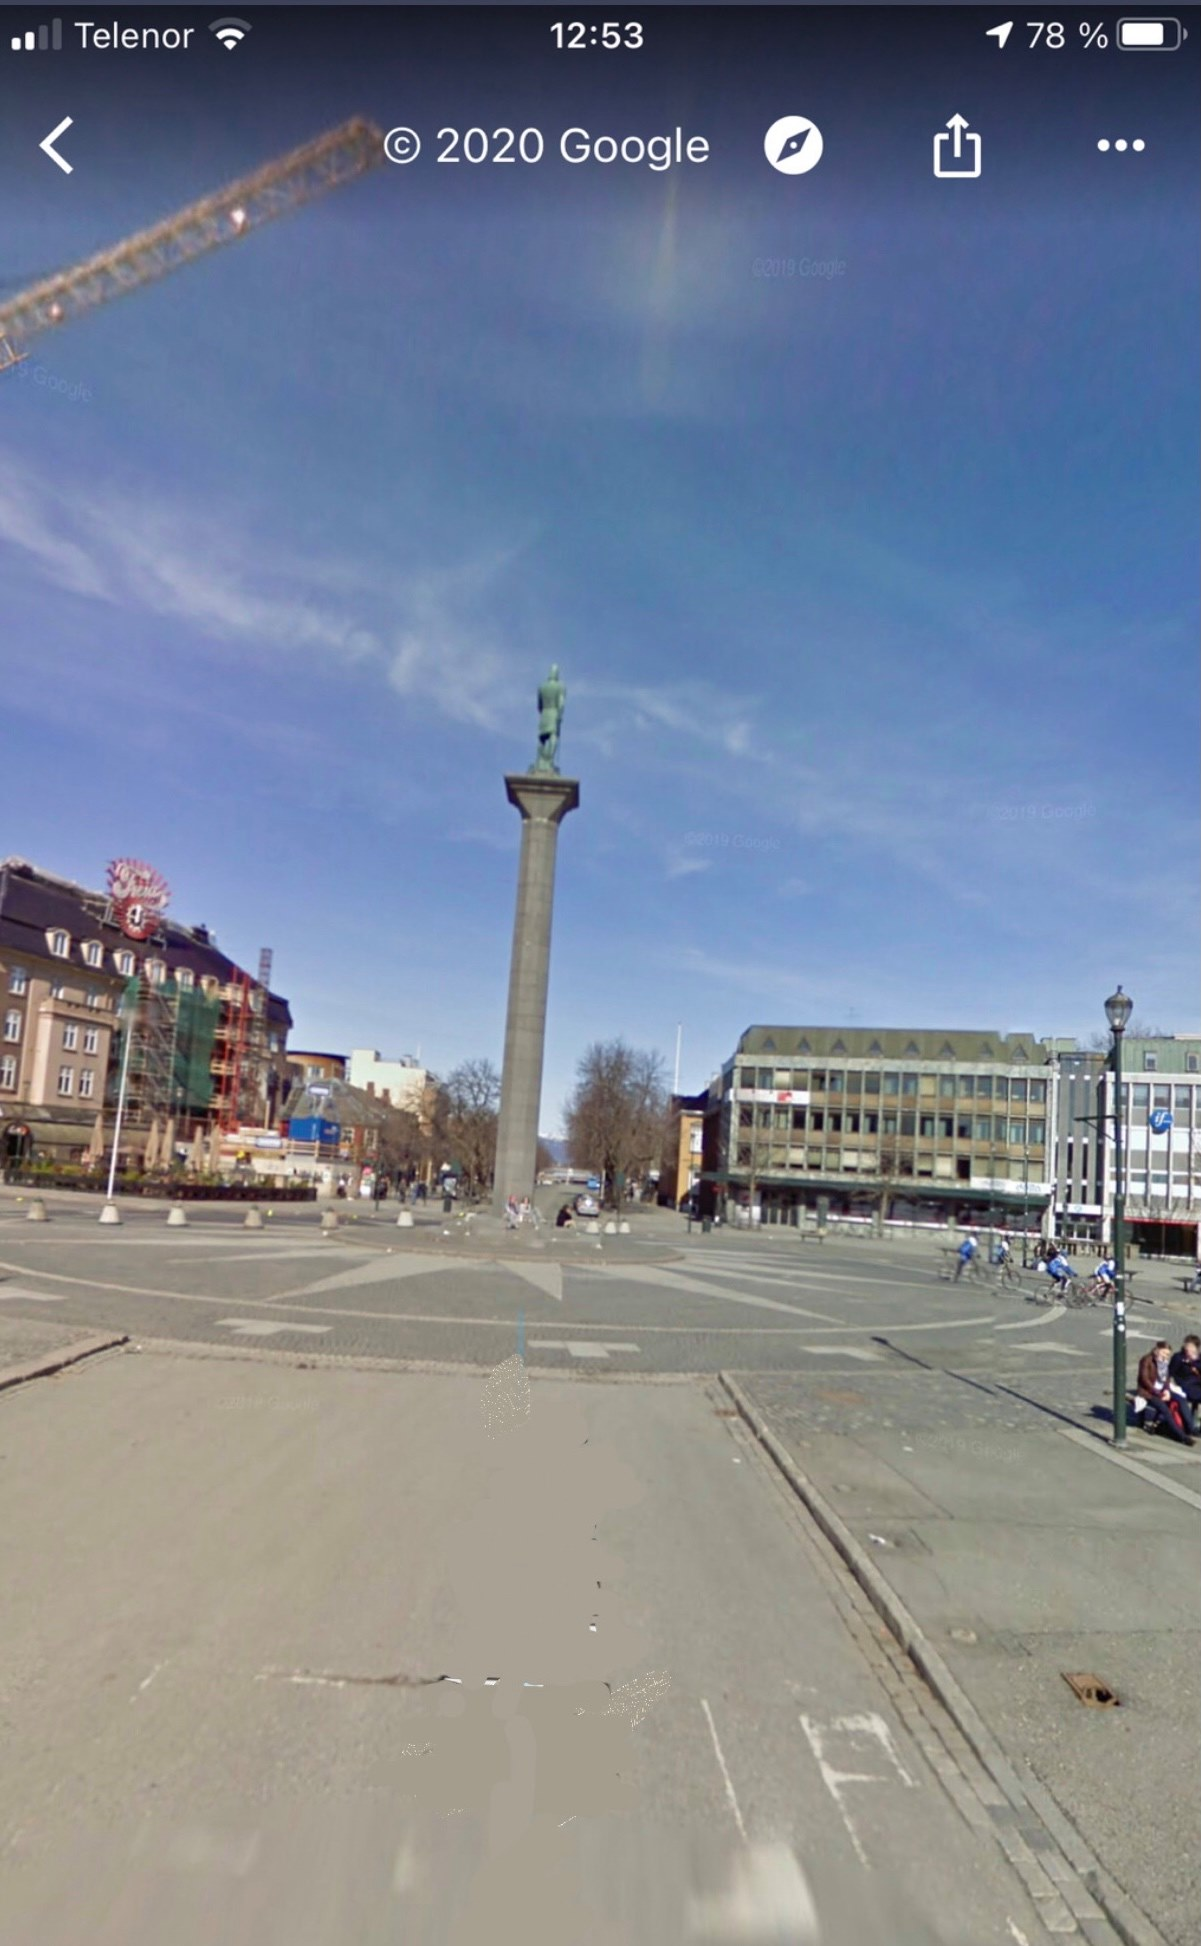
\includegraphics[width=0.48\textwidth]{Images/OurConcepts/streetView.jpg}
              \caption{A street view photo like this photo from Trondheim Torg should give players an indication of where they need to go to complete the challenge in Guess Where.}
              \label{fig:challenge_accepted}
            \end{wrapfigure}

        \subsubsection{Friends Puzzle}

            \begin{wrapfigure}{r}{0.45\textwidth}
                \includegraphics[width=0.4\textwidth]{Images/OurConcepts/teamwork_puzzle.jpg}
                \caption{}
                %\label{fig:}
            \end{wrapfigure}

            \begin{wrapfigure}{l}{0.45\textwidth}
                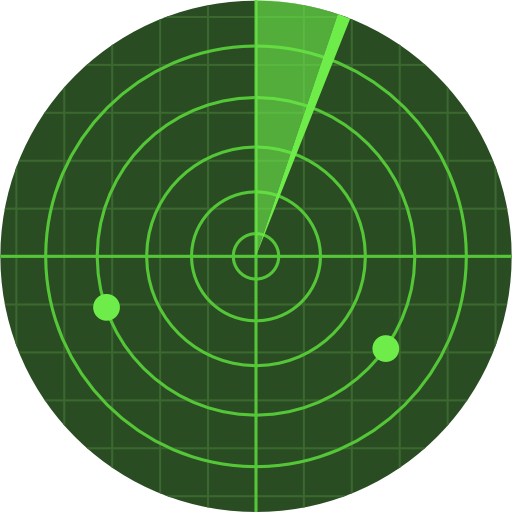
\includegraphics[width=0.4\textwidth]{Images/OurConcepts/radar.png}
                \caption{}
                %\label{fig:}
            \end{wrapfigure}
            
        \subsubsection{Challenge Accepted}
            \begin{figure}[H]
              \centering
              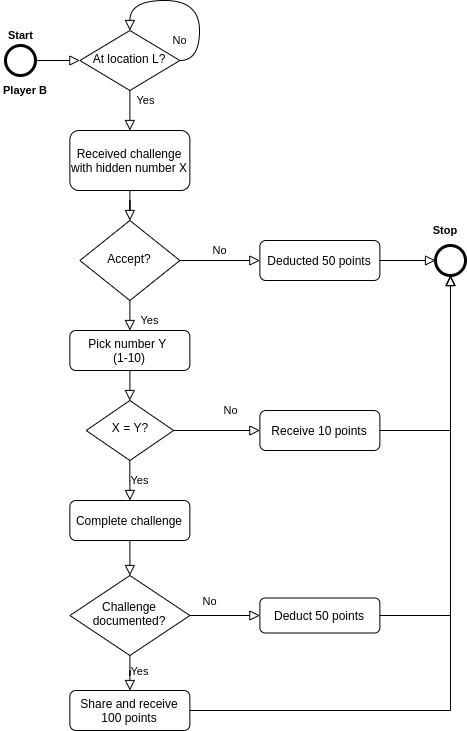
\includegraphics[width=.7\textwidth]{Images/OurConcepts/ChallengeAccepted.png}
              \caption{Player B has to either decline or accept; if the player chooses to decline, he or she will lose 50 points, and if the player chooses to accept, he or she will have to input a number Y between 1 and 10. Then if X is not the same as Y, player B will receive 10 points for being courageous, and will not have to complete the challenge. If X is the same number as Y, player B has to complete the challenge. Also, in order to receive the reward of 100 points, the completion of the challenge has to be documented in the app, and can be shared with friends. }
              \label{fig:challenge_accepted}
            \end{figure}
            
            \begin{wrapfigure}{R}{.45\textwidth}
                \centering
                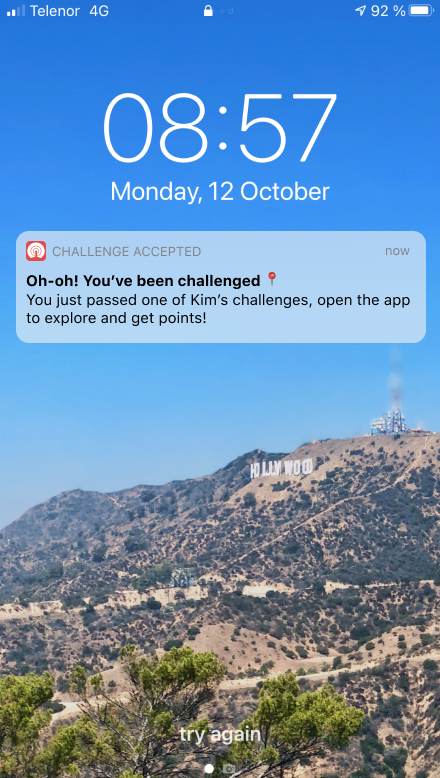
\includegraphics[width=0.4\textwidth]{Images/OurConcepts/ChallengeAcceptedNotification.png}
                \caption{Players get a push notification when they pass a challenge}
                \label{fig:challenge_accepted_notification}
            \end{wrapfigure}
            
            \blindtext   
            
        \subsubsection{Secret Posts}
        
            \begin{figure}[H]
                \begin{minipage}{.5\textwidth}
                  \centering
                  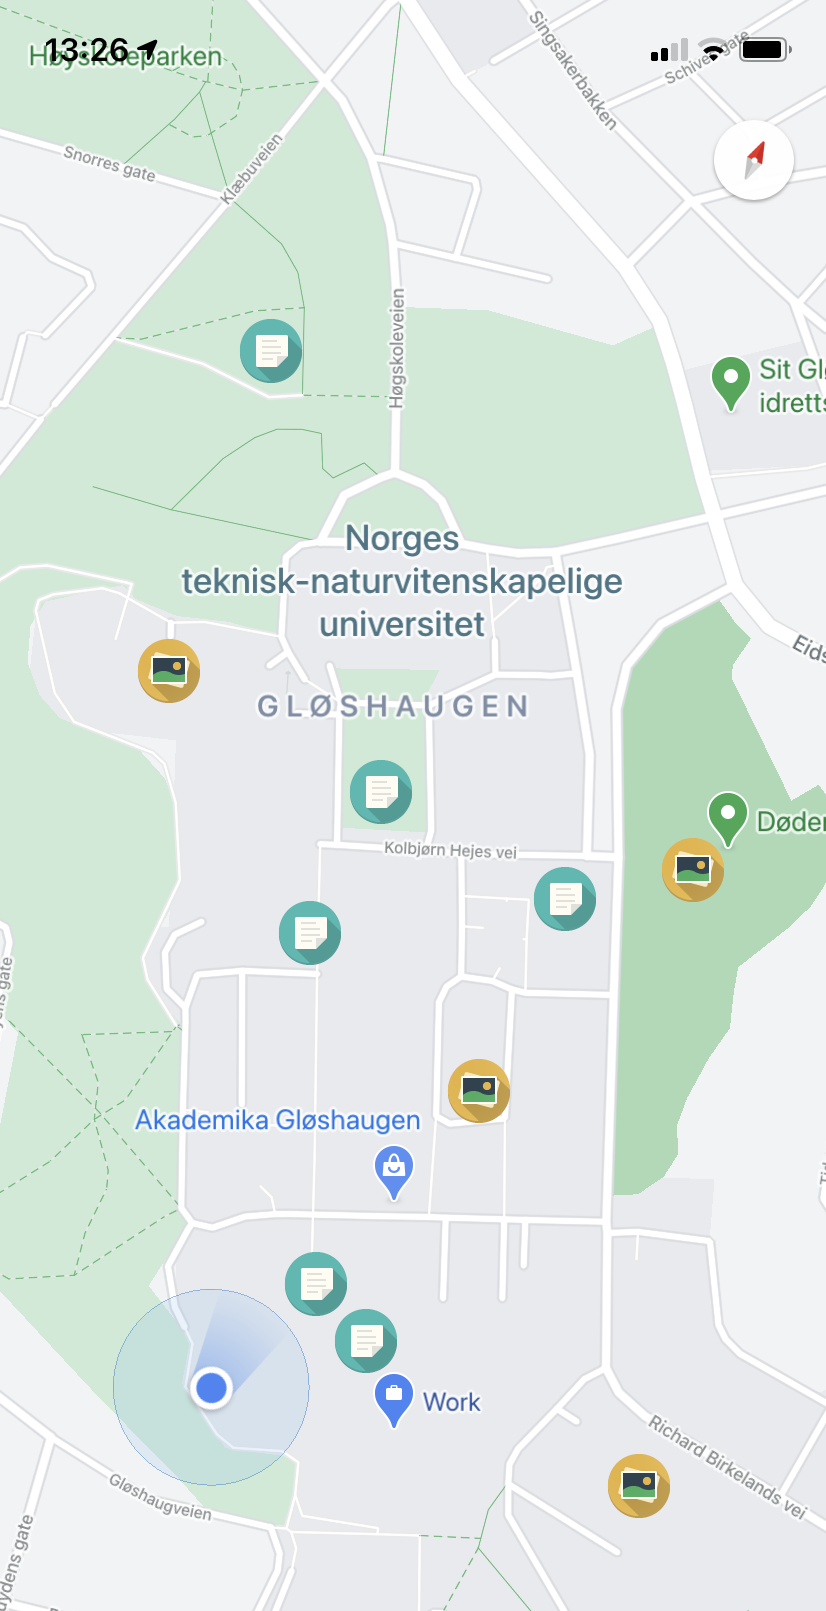
\includegraphics[width=.75\textwidth]{Images/OurConcepts/secret_notes_map.png}
                  \captionof{figure}{The map-view show nearby posts. Each icon indicates location and the type of post.}
                  \label{fig:secret_notes_map}
                \end{minipage}
                \begin{minipage}{.5\textwidth}
                  \centering
                  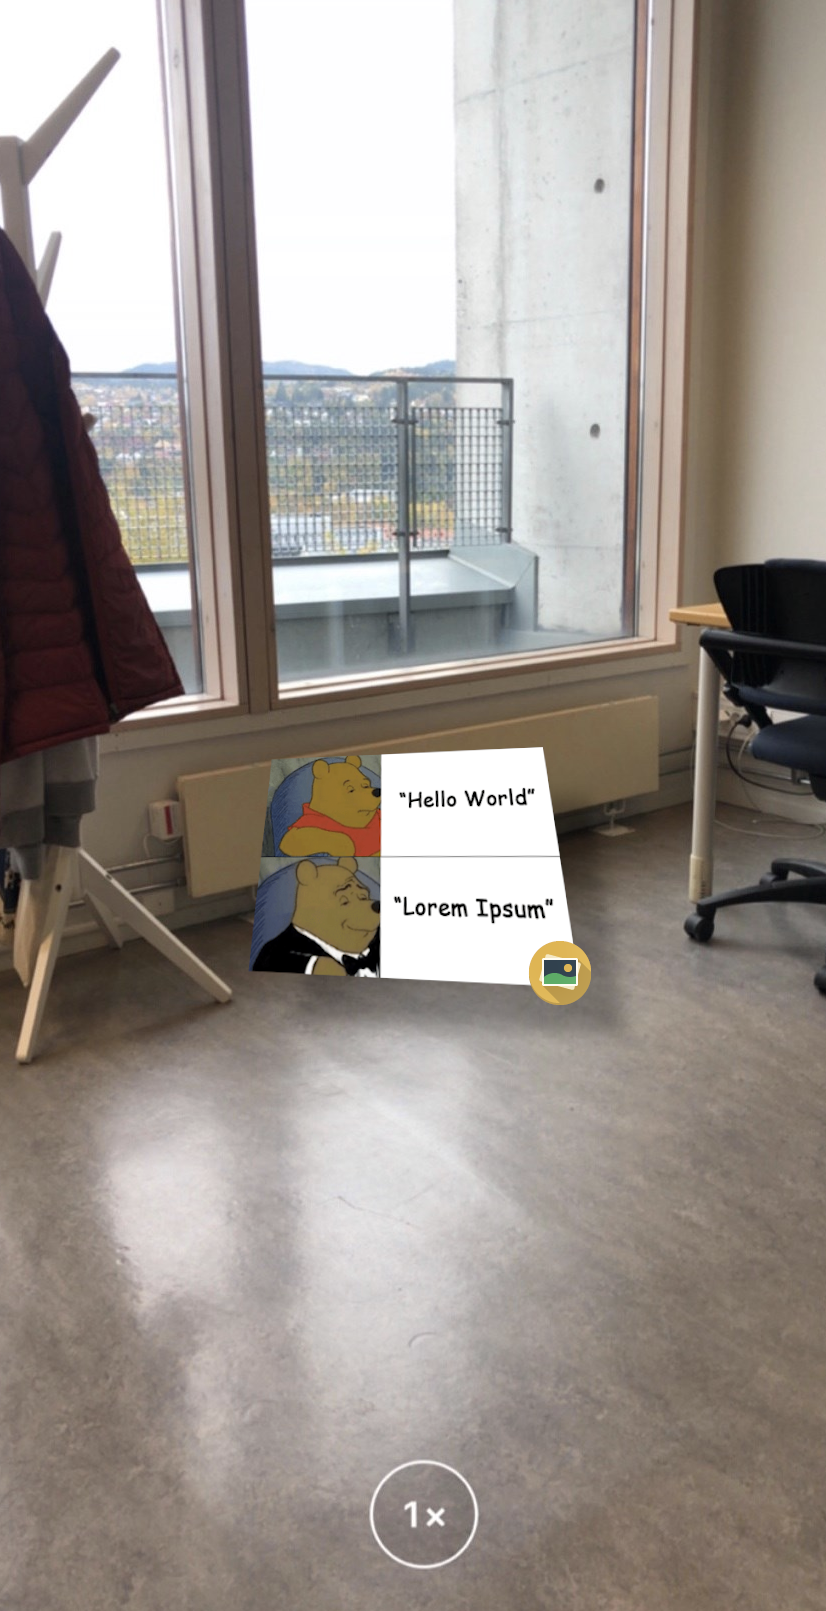
\includegraphics[width=.75\textwidth]{Images/OurConcepts/secret_notes_camera.png}
                  \captionof{figure}{Through the use of AR, players can view the content of the image.}
                  \label{fig:secret_notes_camera}
                \end{minipage}
            \end{figure}
        
        \subsubsection{Free Ticket to Ride}
    \subsection{Comparison}
    
    \begin{figure}[H]
        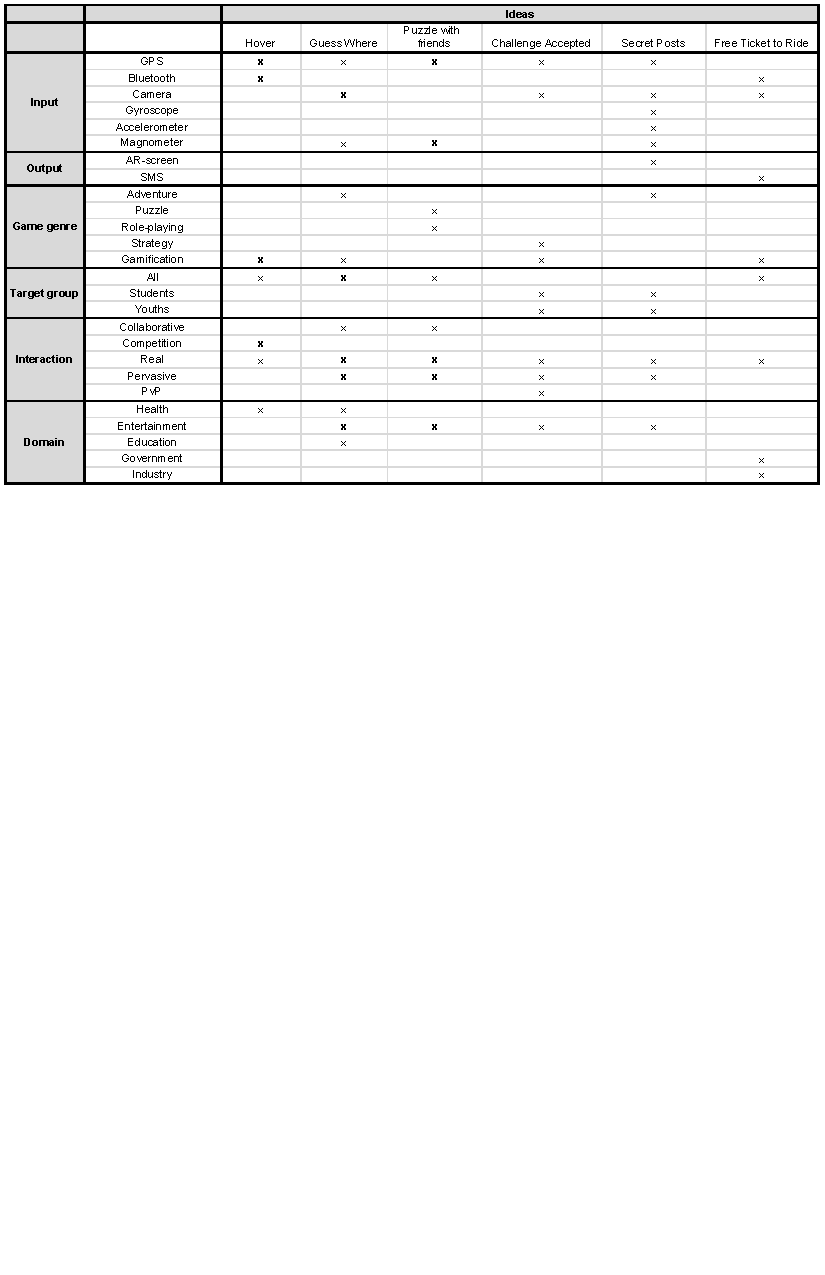
\includegraphics[width=1\textwidth]{Images/Models/OurConceptsS.pdf}
        \caption{Existing alternative games characteristics}
        \label{tab:existing_games}
    \end{figure}
    \subsection{Evaluation}

\biblio % Needed for referencing to working when compiling individual subfiles - Do not remove
\end{document}